\NeedsTeXFormat{LaTeX2e}
\documentclass[10pt,a4]{scrartcl}

\usepackage{tabularx,graphicx,a4,listings,wrapfig,subfigure}

\ifx\pdfoutput\undefined
  % We're not running pdftex
  % european (better) fonts -- does not look good with pdflatex
  \usepackage[T1]{fontenc}
  \newcommand{\href}[2]{#2\\{\hspace*{5mm}\scriptsize <#1>}\\}
\else
  \pdfcompresslevel=9
  \def\pdfBorderAttrs{/Border [0 0 0] } % No border around Links
  \usepackage{hyperref}
\fi

\title{Equalizer Programming Guide\\
  {\footnotesize\mdseries
    \htmladdnormallink{http://www.equalizergraphics.com/documents/Developer/ProgrammingGuide.pdf}
    {http://www.equalizergraphics.com/documents/ProgrammingGuide.pdf}}
}
\author{Stefan Eilemann\thanks{eile@eyescale.ch}\\[\medskipamount]
  % Eyescale Software Sarl
}
\date{
  \textbf{INCOMPLETE}\\[\medskipamount]
  Version 0.7, \today
}

\newcommand{\tm}{\texttrademark~}
\newcommand{\rc}{\raise 1ex\hbox{{\tiny\textregistered}}~}
\newcommand{\fig}[1]{Figure~\ref{#1}}
\newcommand{\link}[1]{\htmladdnormallink{#1}{#1}}

% suppress  single floating lines on top (widow) and bottom(club)
%  10000 is infinity
%  tradeoff: maybe underfull vboxes
\clubpenalty=10000
\widowpenalty=10000 

\begin{document}

\maketitle
\vfill
\lstset{language=C++}

\thispagestyle{empty}
\begin{figure}[ht]
  \hfill
  
\includegraphics[width=4cm]{images/logo.pdf}\hfill
  
\includegraphics[width=4cm]{images/vmml.pdf}\hfill\vspace{-1em}\\
%  {\small\htmladdnormallink{www.eyescale.ch}{http://www.eyescale.ch}}
\end{figure}
\vfill

%\abstract{
%  Equalizer is a project to develop software to simplify the creation of
%  scalable graphics applications and to improve the usability of
%  multipipe visualization systems.
%}


\clearpage
\tableofcontents
\thispagestyle{empty}
\vfill{\center\begin{tabularx}{\textwidth}{|l|l|X|}
    \hline
    \bf Rev & \bf Date     & \bf Changes \\
    \hline
    0.7     & Sep 21, 2007 & started channel and image compositing,
                             added event handling, moved to new eqPly
                             code base\\
    0.6     & Sep 14, 2007 & added pipe, window and object manager\\
    0.5     & Sep 3,  2007 & added config and partly pipe\\
    0.4     & Aug 31, 2007 & added distributed objects\\
    0.3     & Aug 26, 2007 & added application and render client\\
    0.2     & Aug 20, 2007 & added main function\\
    0.1     & Aug 19, 2007 & outlined the basic concepts\\
    \hline
  \end{tabularx}}
\thispagestyle{empty}
\clearpage

\pagenumbering{arabic}



\section{Introduction}

Equalizer provides a framework for the development of parallel
OpenGL\texttrademark\ 
applications. Equalizer-based applications can run a single
shared-memory system with multiple graphics cards (GPU's) or on a
distributed graphics cluster. This Programming Guide introduces the
programming interface using the \textsf{eqPly} example shipped with
Equalizer as a guideline.

Any questions related to Equalizer programming and this Programming
Guide should be directed to the \textsf{eq-dev} mailing
list\footnote{see \link{http://www.equalizergraphics.com/lists.html}}.

Equalizer is the next evolution of a generic parallel programming
interface for visualization applications using OpenGL. Existing
solutions, such as SGI's OpenGL Multipipe\texttrademark\ SDK, VRCO's
Cavelib\texttrademark\ and VRJuggler, implement a subset of concepts
similar to Equalizer. In other areas, e.g., tracking device support,
they provide more functionality.

Equalizer implements the minimum necessary layer to build parallel and
scalable OpenGL applications. The programmer structures the application
so that the OpenGL rendering can be executed in parallel, potentially
across multiple processes for cluster-based execution. Equalizer
provides the domain-specific parallel rendering know-how and abstracts
threading, synchronization, windowing and event handling for
portability. It is a `GLUT on steroids', providing parallel and
distributed execution, scalable rendering features and fully
customizable event handling.

\section{Getting Started}


\subsection{Compiling and running \textsf{eqPly}}

A prerequisite for this Programming Guide is a working \textsf{eqPly}
example. The Quickstart
Guide\footnote{\link{http://www.equalizergraphics.com/documents/EqualizerGuide.html}}
explains how to run it. \textsf{eqPly} can also be executed without a
server, which simplifies the development cycle. In this case it will be
configured to use one window.


\subsection{Equalizer Processes}

\begin{wrapfigure}{r}{.4\textwidth}
  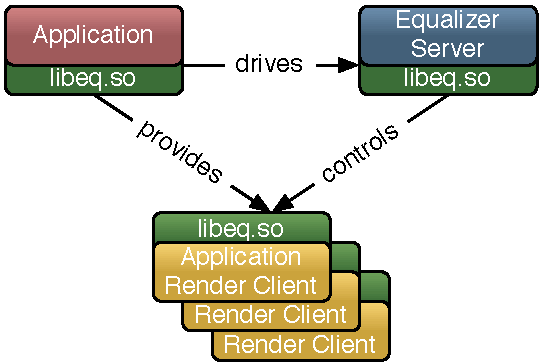
\includegraphics[width=.4\textwidth]{images/processes.pdf}
  {\caption{\small\label{fProcesses}Equalizer Processes}}
\end{wrapfigure}
All functionality of Equalizer is accessed through the Equalizer client
library, which implements all functionality discussed in this document.

\subsubsection{Server}

An Equalizer server is responsible for managing one visualization
system\footnote{a shared memory system or graphics cluster}. Currently
it is only useful for running one application at a time, but it will be
extended to support multiple applications concurrently and efficiently
on one system. The server controls and potentially launches the
application's rendering clients.

\subsubsection{Application}

The application connects to a server, which chooses a configuration for
the application. It provides a render client, to be launched by the
server. The application reacts on events and controls the rendering.

\subsubsection{Render Clients}

The render client implements the rendering part of an application. It is
passive, and receives all its rendering tasks from the server. The tasks
are executed by calling the appropriate task methods (see
\ref{ssTaskMethods}).

The application might be a rendering client, in which case it can also
contribute to the rendering. It can choose not to implement any render
client-related code, in which case it is reduced to be the application's
'master' process without any OpenGL windows.

The rendering client can be the same executable as the application, as
is the case with \textsf{eqPly}. Real-world applications often implement
a separate, light-weight rendering client.



\section{The Programming Interface}

Equalizer uses a C++ programming interface. The API is minimally
invasive, that is, Equalizer imposes only the minimal, natural execution
framework upon the application. It does not impose a scene graph or does
interfere in any way with the application's rendering code.

Methods called by the application always have the form
\textsf{verb[Noun]}, whereas methods called by Equalizer (`Task
Methods') have the form \textsf{nounVerb}.

\subsection{\label{ssTaskMethods}Task Methods}

The application subclasses Equalizer objects and overrides virtual
functions to implement certain functionality, e.g., the application's
OpenGL rendering in \textsf{eq::Chan\-nel::frameDraw}. These task
methods are in concept similar to C function callbacks. The
\textsf{eqPly} section will discuss the most important task methods. A
full list can be found on the
website\footnote{\link{http://www.equalizergraphics.com/documents/design/taskMethods.html}}.


\subsection{The Resource Tree}

The rendering resources are represented in a hierarchical tree structure
which corresponds to the physical and logical resources found in a 3D
rendering environment. 

\begin{figure}[ht!]\center
  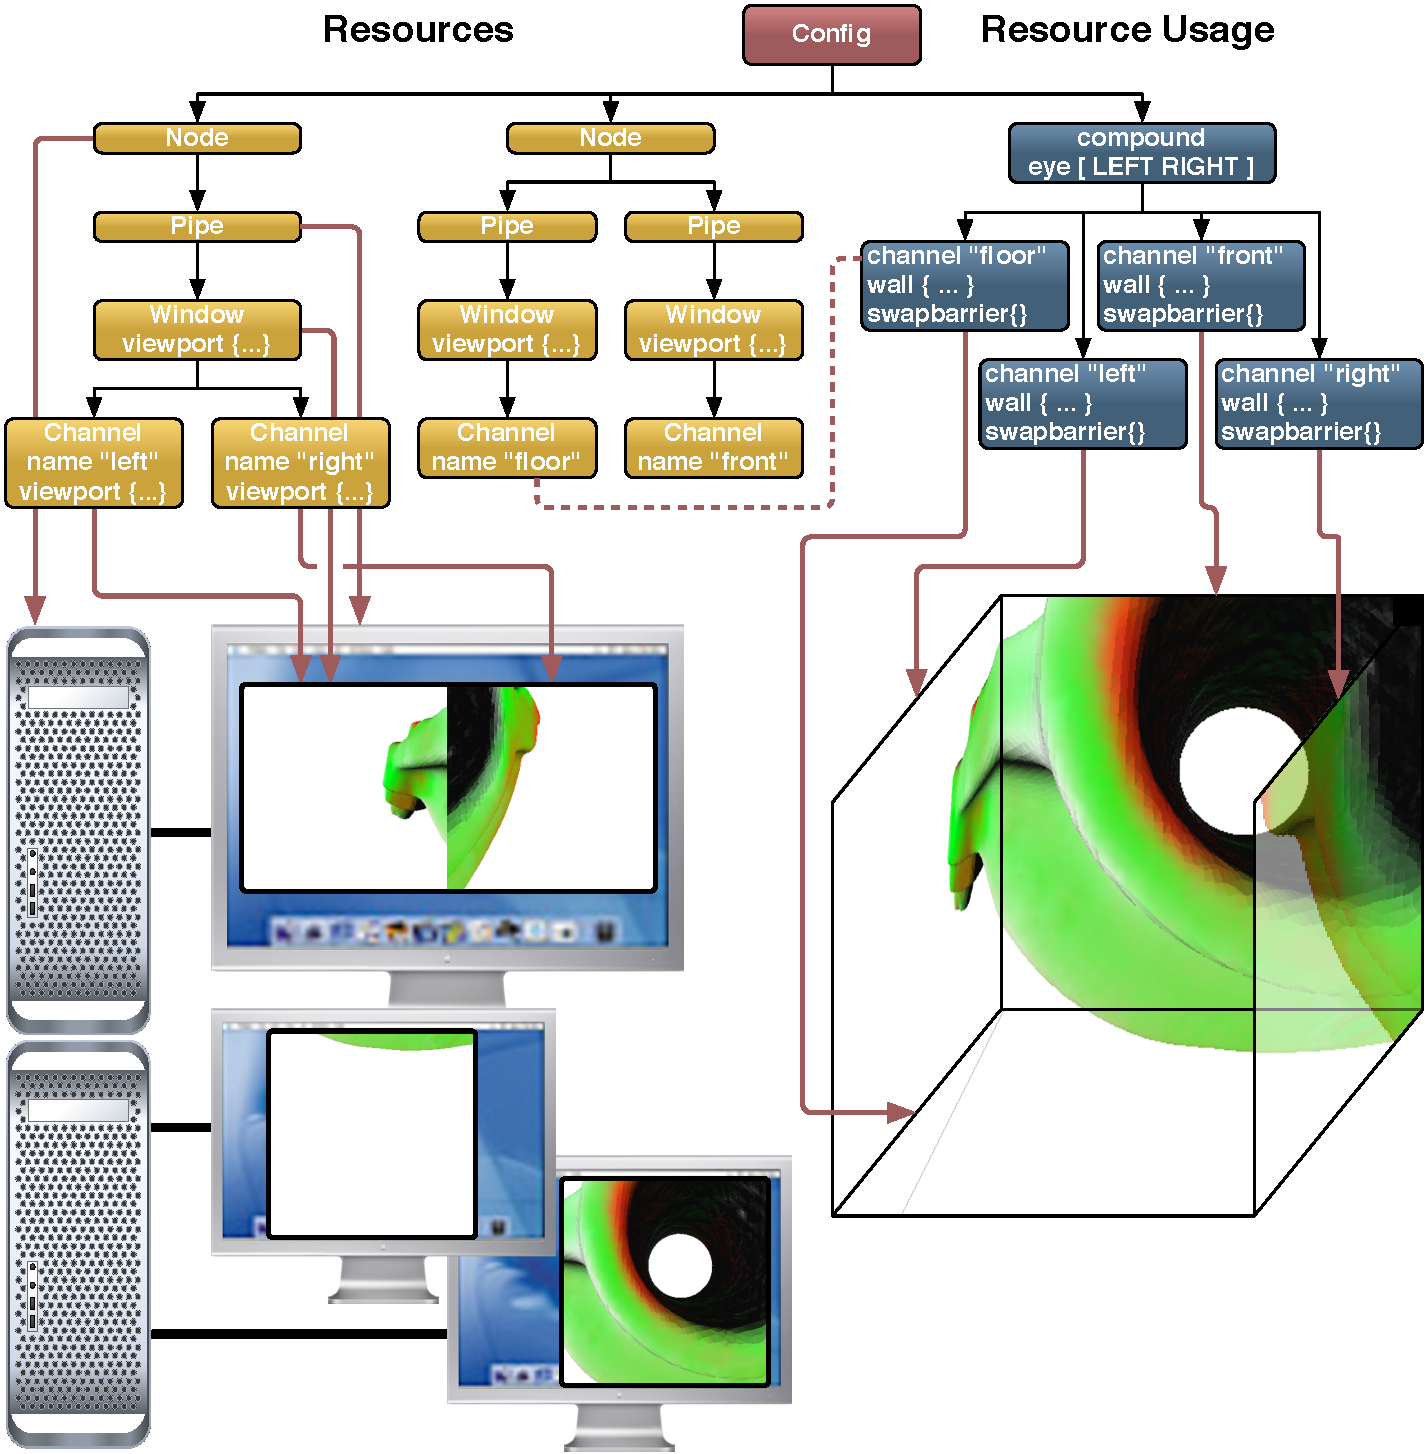
\includegraphics[width=.9\textwidth]{images/cave.pdf}
  {\caption{\small\label{fConfig}An example configuration}}
\end{figure}

\fig{fConfig} shows one example configuration for a four-side
CAVE\texttrademark, running on two machines (node) using three graphics
cards (pipe) with one window each to render to the four output channels
connected to the projectors for each of the walls. The compound
description is only used by the server to compute the rendering
tasks. The application is not aware of compounds, and does not need to
concern itself with the parallel rendering logics of a configuration.

For testing and development purposes it is possible to use multiple
instances for one resource, e.g., to run multiple render client nodes on
one computer. For deployment one node and pipe should be used for each
computer and graphics card, respectively.

\subsubsection{Configuration}

The root of the resource tree is the \textsf{eq::Config}, which
represents the current configuration of the application. It currently
only holds the local node, not all nodes of the configuration.

\subsubsection{Node}

An \textsf{eq::Node} is the representation of a single computer in the
system. It is one operating system process of the render client. All
node task methods are executed from the main application thread. Each
configuration might also use an application node, in which case the
application process is also used for rendering.

\subsubsection{Pipe}

The \textsf{eq::Pipe} is the abstraction of a graphics card (GPU). In
the current implementation it is also one operating system thread,
unless the pipe's thread hint is set to \textsf{false}. All pipe and
child window and channel task methods are executed from the pipe thread
for threaded pipes or from the main application thread for non-threaded
pipes\footnote{see also
  \link{http://www.equalizergraphics.com/documents/design/nonthreaded.html}}.

Further versions of Equalizer might introduce threaded windows, where
all window-related task methods are executed in a separate operating
system thread.

\subsubsection{Window}

An \textsf{eq::Window} is an drawable and OpenGL context. The drawable
can be an on-screen window or an off-screen PBuffer or
FBO\footnote{off-screen drawables are not yet implemented, but can be
  created by the application and used with Equalizer}. 

\subsubsection{Channel}

The \textsf{eq::Channel} is the abstraction of an OpenGL viewport within
its parent window. It is the entity executing the actual rendering.


\subsection{Resource Usage}

How the rendering resources are to be used is configured using a
compound tree. Each compound has a channel, which it uses to execute the
rendering tasks. The rendering tasks are computed by the server and send
to the render clients. At no point the application or render clients
have or need knowledge of compounds. The configuration of compounds is
not in the scope of this document\footnote{see
  \link{http://www.equalizergraphics.com/documents/design/compounds.html}}.



\section{The \textsf{eqPly} polygonal renderer}

The \textsf{eqPly} example is shipped with the Equalizer distribution
and serves as a simple reference implementation of an Equalizer-based
application. Its focus is not on rendering features or visual quality.
It serves as a test bed for most of the Equalizer features.

In this section the source code of \textsf{eqPly} is discussed in
detail, and relevant design decision and remarks are raised.

All classes in the example are in the \textsf{eqPly} namespace to avoid
type name ambiguities, in particular for the \textsf{Window} class.


\subsection{The main Function}

The main function starts off with parsing the command line into the
\textsf{LocalInitData} data structure, which in part will be distributed
to all render client nodes. For actual command line parsing is done by
the \textsf{LocalInitData} class and will be discussed there:

{\footnotesize\begin{lstlisting}
int main( int argc, char** argv )
{
    // 1. parse arguments
    eqPly::LocalInitData initData;
    initData.parseArguments( argc, argv );
\end{lstlisting}}

The second step is to initialize the Equalizer library. The
initialization function of Equalizer also parses the command line, which
is used to set certain default values based on Equalizer-specific
options\footnote{Equalizer-specific options always start with -\,-eq-},
e.g., the default server location. Furthermore, a node factory is
provided. The \textsf{EQERROR} macro, and its counterparts
\textsf{EQWARN}, \textsf{EQINFO} and \textsf{EQVERB} allow selective
debugging outputs with various logging levels:

{\footnotesize\begin{lstlisting}
    // 2. Equalizer initialization
    NodeFactory nodeFactory;
    if( !eq::init( argc, argv, &nodeFactory ))
    {
        EQERROR << "Equalizer init failed" << endl;
        return EXIT_FAILURE;
    }
\end{lstlisting}}%>>

The node factory is used by Equalizer to create the object instances for
the rendering entities. Each of the classes inherits from the same type
provided by Equalizer in the \textsf{eq} namespace. The provided
\textsf{eq::NodeFactory} base class instantiates a 'plain' Equalizer
object, thus making it possible to selectively subclass individual
entity types. For each rendering resource used in the configuration, one
C++ object will be created:

{\footnotesize\begin{lstlisting}
class NodeFactory : public eq::NodeFactory
{
public:
    virtual eq::Config*  createConfig()  { return new eqPly::Config; }
    virtual eq::Node*    createNode()    { return new eqPly::Node; }
    virtual eq::Pipe*    createPipe()    { return new eqPly::Pipe; }
    virtual eq::Window*  createWindow()  { return new eqPly::Window; }
    virtual eq::Channel* createChannel() { return new eqPly::Channel; }
};
\end{lstlisting}}

The third step is to create an instance of the application and to
initialize it locally. The application is an \textsf{eq::Client}, which
is an \textsf{eqNet::Node}. The underlying network distribution in
Equalizer is a peer-to-peer network structure of
\textsf{eqNet::Node}s. The application programmer rarely is aware of the
classes in the \textsf{eqNet} namespace, but both the
\textsf{eq::Client} and the server are \textsf{eqNet::Node}s. The local
initialization of nodes creates a local listening socket, so that the
node, and therefore the \textsf{eq::Client} can communicate over the
network with other nodes, such as the server and the rendering clients.

{\footnotesize\begin{lstlisting}
    // 3. initialization of local client node
    RefPtr< eqPly::Application > client = new eqPly::Application( initData );
    if( !client->initLocal( argc, argv ))
    {
        EQERROR << "Can't init client" << endl;
        eq::exit();
        return EXIT_FAILURE;
    }
\end{lstlisting}}%>>

Finally everything is set up to run the \textsf{eqPly} application:

{\footnotesize\begin{lstlisting}
    // 4. run client
    const int ret = client->run();
\end{lstlisting}}

After it has finished, the application and Eqply is deinitialized and
the \textsf{main} function returns:

{\footnotesize\begin{lstlisting}
    // 5. cleanup and exit
    client->exitLocal();
    client = 0;

    eq::exit();
    return ret;
}
\end{lstlisting}}


\subsection{Application}

In the \textbf{eqPly} case, the application is also the render client. It has
three run-time behaviours:

\begin{enumerate}
  \item \textbf{Application}: The executable started by the user, which
    is the controlling entity in the rendering session.
  \item \textbf{Auto-launched render client}: The typical render client,
    started by the server. The server starts the executable with special
    parameters, which cause \textsf{Client::initLocal} to never
    return. During exit, the server terminates the process.
  \item \textbf{Resident render client}: Manually pre-started render
    client, listening on a specified port for server commands. This mode
    is selected using the command-line option \textsf{--eq-client} and
    potentially \textsf{--eq-listen} and \textsf{-r}\footnote{see \link{http://www.equalizergraphics.com/documents/design/residentNodes.html}}.
\end{enumerate}

\subsubsection{Main Loop}

The application's main loop starts by connecting the application to an
Equalizer server. The command line parameter \textsf{--eq-server}
explicitly specifies a server address. If no server was specified,
\textsf{Client::connectServer} try first to connect to a server on the
local machine using the default port 4242. If that fails, it will create
a server running within the applications process with a default
1-channel configuration\footnote{see
  \link{http://www.equalizergraphics.com/documents/design/standalone.html}}.

{\footnotesize\begin{lstlisting}
int Application::run()
{
    // 1. connect to server
    RefPtr<eq::Server> server = new eq::Server;
    if( !connectServer( server ))
    {
        EQERROR << "Can't open server" << endl;
        return EXIT_FAILURE;
    }
\end{lstlisting}}%>>

The second step is to ask the server for a configuration. The
\textsf{ConfigParams} are a placeholder for later implementations to
provide additional hints and information to the server for choosing a
configuration. The configuration is created using
\textsf{NodeFactory::createConfig}. Therefore it is of type
\textsf{eqPly::Config}, but the return value is \textsf{eq::Config},
making q cast necessary:

{\footnotesize\begin{lstlisting}
    // 2. choose config
    eq::ConfigParams configParams;
    Config* config = static_cast<Config*>(server->chooseConfig( configParams ));

    if( !config )
    {
        EQERROR << "No matching config on server" << endl;
        disconnectServer( server );
        return EXIT_FAILURE;
    }
\end{lstlisting}}%>>

Finally it is time to initialize the configuration. For statistics, the
time for this operation is measures and printed. During initialization
the server launches and connects all render client nodes, and calls the
appropriate initialization task methods, as explained in later
sections. \textsf{Config::init} does return after all nodes, pipes,
windows and channels are initialized. It returns \textsf{true} only if
all init task methods were successful. The \textsf{EQLOG} macro allows
topic-specific logging. The numeric topic values are specified in the
respective \textsf{log.h} header files:

{\footnotesize\begin{lstlisting}
    // 3. init config
    eqBase::Clock clock;

    config->setInitData( _initData );
    if( !config->init( ))
    {
        EQERROR << "Config initialization failed: " 
                << config->getErrorMessage() << endl;
        server->releaseConfig( config );
        disconnectServer( server );
        return EXIT_FAILURE;
    }

    EQLOG( eq::LOG_CUSTOM ) << "Config init took " << clock.getTimef() << " ms"
                            << endl;
\end{lstlisting}}%>>

When the configuration was successfully initialized, the actual main
loop is executed. The main loop runs until the user exits the
configuration or a maximum number of frames, specified as a command-line
argument, has been rendered. The latter is useful for benchmarks. The
\textsf{Clock} is reused for measuring the overall performance. A new
frame is started using \textsf{Config::startFrame} and a frame is
finished using \textsf{Config::finishFrame}.

When the frame is started, the server computes all rendering tasks and
sends them to the appropriate render client nodes. The render client
nodes dispatch the tasks to the correct node or pipe thread, were they
are executed in the order they arrive.

\begin{wrapfigure}{r}{.6\textwidth}
  \subfigure[]{\label{fSync}
    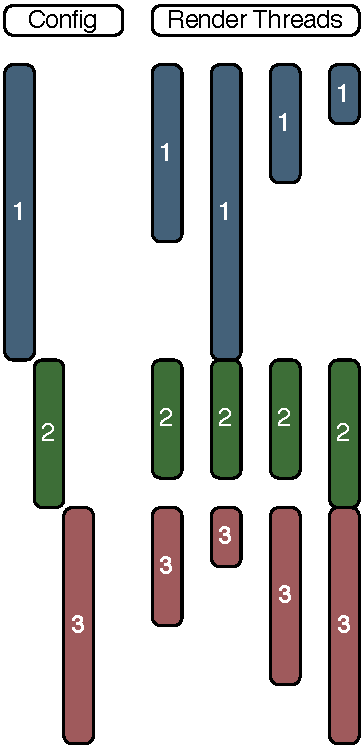
\includegraphics[width=.25\textwidth]{images/sync}}\hfil
  \subfigure[]{\label{fAsync}
    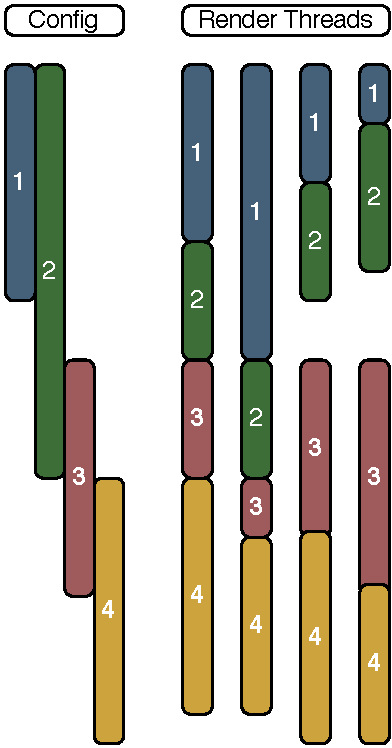
\includegraphics[width=.25\textwidth]{images/async}}%
  {\caption{\small\label{fSyncAsync}Synchronous and asynchronous execution}}
\end{wrapfigure}
\textsf{Config::finishFrame} synchronizes on the completion of the frame
\textsf{current - latency}. The latency is specified in the
configuration file, and allows several outstanding frames for which the
tasks are already queued in the node and pipe threads for
execution. This enables overlapped execution and minimizes idle
times. The first \textsf{latency Config::finishFrame} return
immediately, since they have no frame to synchronize
upon. \fig{fSyncAsync} shows the execution of (hypothetical)
rendering tasks without latency~(\fig{fSync}) and with a latency of
one~(\fig{fAsync}).

When the main loop is finished, \textsf{Config::finishAllFrames} catches
up with the latency. It returns after all outstanding frames have been
rendered, and is needed here to provide an accurate measurement of the
framerate:

{\footnotesize\begin{lstlisting}
    // 4. run main loop
    uint32_t maxFrames = _initData.getMaxFrames();
    
    clock.reset();
    while( config->isRunning( ) && maxFrames-- )
    {
        config->startFrame();
        // config->renderData(...);
        config->finishFrame();
    }
    const uint32_t frame = config->finishAllFrames();
    const float    time  = clock.getTimef();
    EQLOG( eq::LOG_CUSTOM ) << "Rendering took " << time << " ms (" << frame
                            << " frames @ " << ( frame / time * 1000.f)
                            << " FPS)" << endl;
\end{lstlisting}}%>>

The remainder of the application code cleans up in the reverse order of
the initialization. The config is exited, released and the connection to
the server is closed:

{\footnotesize\begin{lstlisting}
    // 5. exit config
    clock.reset();
    config->exit();
    EQLOG( eq::LOG_CUSTOM ) << "Exit took " << clock.getTimef() << " ms" <<endl;

    // 6. cleanup and exit
    server->releaseConfig( config );
    if( !disconnectServer( server ))
        EQERROR << "Client::disconnectServer failed" << endl;
    server = 0;
    return EXIT_SUCCESS;
}
\end{lstlisting}}%>>

\subsubsection{Render Clients}

In the second and third case, when the executable is used as a render
client, \textsf{Client::initLocal} never returns. Therefore the
application's main loop is never executed. In order to keep the client
resident, the \textsf{eqPly} example overrides the client loop to keep
it running beyond one configuration run:

{\footnotesize\begin{lstlisting}
bool Application::clientLoop()
{
    if( !_initData.isResident( )) // execute only one config run
        return eq::Client::clientLoop();

    // else execute client loops 'forever'
    while( true ) // TODO: implement SIGHUP handler to exit?
    {
        if( !eq::Client::clientLoop( ))
            return false;
        EQINFO << "One configuration run successfully executed" << endl;
    }
    return true;
}
\end{lstlisting}}%>>


\subsection{Distributed Objects}

Equalizer provides distributed objects which help implementing data
distribution in a graphics cluster. The master version of a distributed
object is registered with a \textsf{eqNet::Session}, which assigns a
session-unique identifier to the object. Other nodes can map their
instance of the object to this identifier, thus synchronizing the
object's data with the remotely registered object.

Distributed object are created by subclassing from
\textsf{eqNet::Object}. Distributed objects can be static (immutable) or
dynamic. Dynamic objects are versioned.

The \textsf{eqPly} example has a static distributed object to provide
initial data to all rendering nodes, as well as a versioned object to
provide frame-specific data, such as the camera position, to the
rendering methods.

\subsubsection{InitData - a Static Distributed Object}

The \textsf{InitData} class holds a couple of parameters needed during
initialization. These parameters never change during one configuration
run, and are therefore static.

A static distributed object either has to provide a pointer and size to
its data using \textsf{setInstanceData} or it has to implement
\textsf{getInstanceData} and \textsf{applyInstanceData}. The first
approach can be used if all distributed member variables can be outlayed
in one contiguous block of memory. The second approach is used
otherwise.

The \textsf{InitData} class contains a string of variable
length. Therefore it uses the second approach of manually serializing
and deserializing its data. The serialization is done in
\textsf{getInstanceData}. The serialized data is cached using a
(non-distributed) member variable, which is cleared by each setter of
distributed data. Serializing the data is a simple matter of allocating
a large enough memory buffer, and copying the data into the buffer:

{\footnotesize\begin{lstlisting}
const void* InitData::getInstanceData( uint64_t* size )
{
    *size = sizeof( StaticData ) + _filename.length() + 1;
    if( _instanceData )
        return _instanceData;

    _instanceData = new char[ *size ];

    reinterpret_cast< StaticData* >( _instanceData )[0] = _data;

    const char* string = _filename.c_str();
    memcpy( _instanceData + sizeof( StaticData ), string, _filename.length()+1);

    return _instanceData;
}
\end{lstlisting}}

After the data is no longer needed, \textsf{releaseInstanceData} is
called by Equalizer to allow the object to free the data. Since the data
is cached for further usage, the release method is not overwritten in
\textsf{InitData}.

The memory buffer returned by \textsf{getInstanceData} is transferred to
the remote node during object mapping and passed to
\textsf{applyInstanceData} for deserialization. The deserialization
routine reads the data back into its own member variables:

{\footnotesize\begin{lstlisting}
void InitData::applyInstanceData( const void* data, const uint64_t size )
{
    _data     = reinterpret_cast< const StaticData* >( data )[0];
    _filename = static_cast<const char*>( data ) + sizeof( StaticData );

    EQASSERT( _data.frameDataID != EQ_ID_INVALID );
    EQINFO << "New InitData instance" << endl;
}
\end{lstlisting}}%>>

\subsubsection{FrameData - a Versioned Distributed Object}

Versioned objects have to override \textsf{isStatic} to return false, in
order for Equalizer to know that they should be versioned. Right now,
only the master instance of the object is writable, that is,
\textsf{eqNet::Object::commit} can be called to generate a new
version. 

Upon \textsf{commit} the delta data from the previous version is sent to
all mapped slave instances. The data is queued on the remote node, and
is applied when the application calls \textsf{sync} to synchronize the
object to a new version. The \textsf{sync} method might block if a
version has not been committed or is still in transmission.

In addition to the instance data (de)serialization methods needed to map
an object, versioned objects may implement \textsf{pack} and
\textsf{unpack} to serialize or deserialize the changes since the last
version.

If the delta data happens to be layed out contiguously in memory,
\textsf{setDeltaData} might be used. The default implementation of
\textsf{pack} and \textsf{unpack} (de)serialize the delta data or the
instance data if no delta data has been specified.

The frame data is layed out in one anonymous structure in
memory. It also does not track changes since it is relatively small in
size and changes frequently. Therefore, for the instance and delta
date are the same and set in the constructor:

{\footnotesize\begin{lstlisting}
        FrameData()
            {
                reset();
                setInstanceData( &data, sizeof( Data ));
                EQINFO << "New FrameData " << std::endl;
            }
\end{lstlisting}}%>>

\subsection{Config}

The configuration is driving the applications rendering, that is, it is
responsible for updating the data based on received events, requesting
new frames to be rendered and to provide the render clients with the
necessary data.

\subsubsection{Initialization and Exit}

\begin{wrapfigure}{r}{.6\textwidth}
  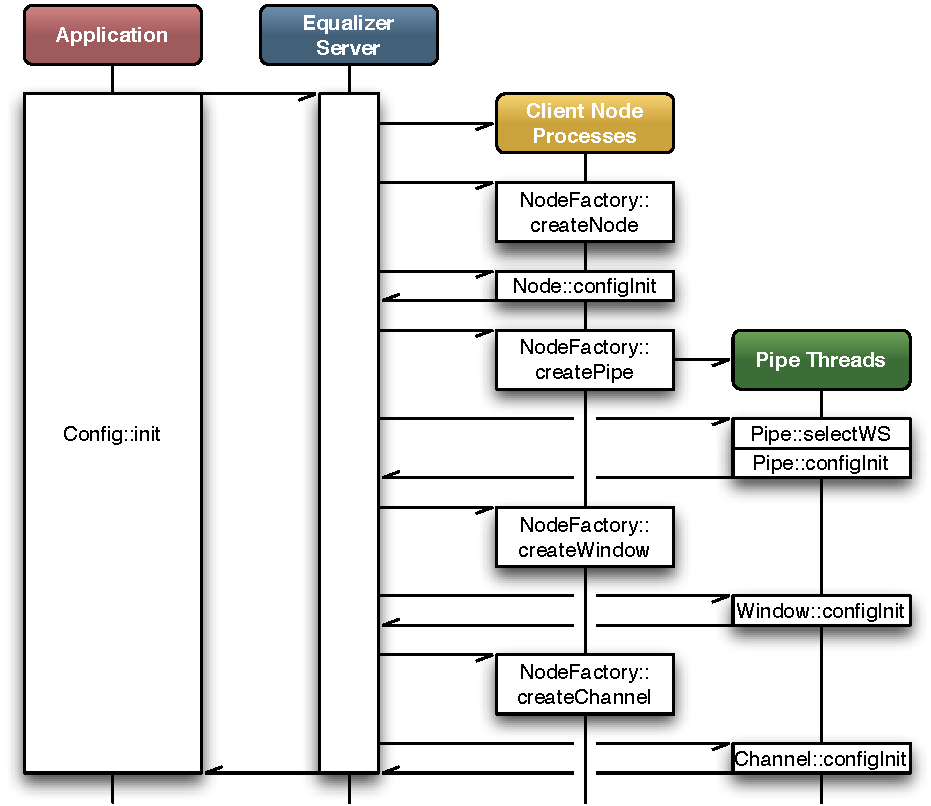
\includegraphics[width=.6\textwidth]{images/configInit.pdf}
  {\caption{\small\label{fConfigInit}Config Initialization Sequence}}
\end{wrapfigure}
The config initialization happens in parallel, that is, all config
initialization tasks are transmitted by the server at once and their
execution is synchronized later. 

The tasks are executed by the node and pipe threads in parallel. The
parent's initialization methods are always executed before any child
initialization method. This is necessary to allow a speedy startup of
the configuration on large-scale graphics clusters. On the other hand,
it means that initialization functions are called even if the parent's
initialization has failed.

The \textsf{eqPly::Config} class holds the master versions of the
initialization and frame data. Both objects are registered with the
\textsf{eq::Config}, which is the \textsf{eqNet::Session} used for
rendering. Equalizer takes care of the session setup and exit in
\textsf{Client::choose\-Config} and \textsf{Client::releaseConfig},
respectively.

The frame data is registered first, since its identifier is transmitted
using the initialization data, which is registered afterwards. The
identifier of the initialization data is transmitted to the render
client nodes using the \textsf{initID} parameter of
\textsf{eq::Config::init}. Equalizer will pass this identifier to all
\textsf{configInit} calls of the respective objects:

{\footnotesize\begin{lstlisting}
bool Config::init()
{
    // init distributed objects
    _frameData.data.color = _initData.useColor();
    registerObject( &_frameData );
    _initData.setFrameDataID( _frameData.getID( ));

    registerObject( &_initData );

    // init config
    _running = eq::Config::init( _initData.getID( ));
    if( !_running )
        return false;
\end{lstlisting}}

If the configuration was initialized correctly, the configuration tries
to set up a tracking device for head tracking. Equalizer does not
provide extensive support for tracking device, as this is an orthogonal
problem to parallel rendering, and has been solved already by a number
of implementations\footnote{VRCO Trackd, VRPN, etc.}. The example
code in \textsf{eqPly} is one reference implementation for the
integration of such a tracking library:

{\footnotesize\begin{lstlisting}
    // init tracker
    if( !_initData.getTrackerPort().empty( ))
    {
        if( !_tracker.init( _initData.getTrackerPort() ))
            EQWARN << "Failed to initialise tracker" << endl;
        else
        {
            // Set up position of tracking system in world space
            // Note: this depends on the physical installation.
            vmml::Matrix4f m( vmml::Matrix4f::IDENTITY );
            m.scale( 1.f, 1.f, -1.f );
            //m.x = .5;
            _tracker.setWorldToEmitter( m );

            m = vmml::Matrix4f::IDENTITY;
            m.rotateZ( -M_PI_2 );
            _tracker.setSensorToObject( m );
            EQLOG( eq::LOG_CUSTOM ) << "Tracker initialised" << endl;
        }
    }

    return true;
}
\end{lstlisting}}%>>

The exit of the configuration stops the render clients by calling
\textsf{eq::Config::exit}, and then deregisters the initialization and
frame data objects with the session:

{\footnotesize\begin{lstlisting}
bool Config::exit()
{
    _running = false;
    const bool ret = eq::Config::exit();

    _initData.setFrameDataID( EQ_ID_INVALID );
    deregisterObject( &_initData );
    deregisterObject( &_frameData );

    return ret;
}
\end{lstlisting}}

\subsubsection{Frame Control}

The rendering frames are issued by the application. The \textsf{Config}
only overrides \textsf{startFrame} in order to update the its data
before forwarding the start frame request to the \textsf{eq::Config}.

If a tracker is used, the current head position and orientation is
retrieved and given to Equalizer, which uses the head matrix together
with the wall or projection description to compute the view
frustra\footnote{see
  \link{http://www.equalizergraphics.com/documents/design/immersive.html}}.

The camera position is updated and the frame data is commited, which
generates a new version. This version is passed to the rendering
callbacks and will be used to synchronize the frame data to the state
belonging to the current frame:

{\footnotesize\begin{lstlisting}
uint32_t Config::startFrame()
{
    // update head position
    if( _tracker.isRunning() )
    {
        _tracker.update();
        const vmml::Matrix4f& headMatrix = _tracker.getMatrix();
        setHeadMatrix( headMatrix );
    }

    // update database
    _frameData.data.rotation.preRotateX( -0.001f * _spinX );
    _frameData.data.rotation.preRotateY( -0.001f * _spinY );
    const uint32_t version = _frameData.commit();

    return eq::Config::startFrame( version );
}
\end{lstlisting}}

\subsubsection{Event Handling}

Events are send by the render clients to the application using
\textsf{eq::Config::sendEvent}. At the end of the frame,
\textsf{Config::finishFrame} calls \textsf{Config::handleEvents} to do
the event handling. The default implementation processes all pending
events by calling \textsf{Config::handleEvent} for each of them.

For event-driven execution, the application can override
\textsf{Config::handleEvents} to blockingly receive events using
\textsf{Config::nextEvent} until a new frame has to be rendered.

The \textsf{eqPly} example continuously renders new frames. It
implements \textsf{Config::hand\-le\-Event} to provide the various reactions
to user input, most importantly camera updates based on mouse
events. The camera position has to be handled correctly with respect to
latency, and is therefore saved in the frame data:

{\footnotesize\begin{lstlisting}
bool Config::handleEvent( const eq::ConfigEvent* event )
{
    switch( event->type )
    {
        case eq::ConfigEvent::WINDOW_CLOSE:
            _running = false;
            return true;

        [...]

        case eq::ConfigEvent::POINTER_MOTION:
            if( event->pointerMotion.buttons == eq::PTR_BUTTON_NONE )
                return true;

            if( event->pointerMotion.buttons == eq::PTR_BUTTON1 )
            {
                _spinX = 0;
                _spinY = 0;

                _frameData.data.rotation.preRotateX( 
                    -0.005f * event->pointerMotion.dx );
                _frameData.data.rotation.preRotateY(
                    -0.005f * event->pointerMotion.dy );
            }
            else if( event->pointerMotion.buttons == eq::PTR_BUTTON2 ||
                     event->pointerMotion.buttons == ( eq::PTR_BUTTON1 |
                                                       eq::PTR_BUTTON3 ))
            {
                _frameData.data.translation.z +=
                    .005f * event->pointerMotion.dy;
            }
            else if( event->pointerMotion.buttons == eq::PTR_BUTTON3 )
            {
                _frameData.data.translation.x += 
                    .0005f * event->pointerMotion.dx;
                _frameData.data.translation.y -= 
                    .0005f * event->pointerMotion.dy;
            }
            return true;

        default:
            break;
    }
    return eq::Config::handleEvent( event );
}
\end{lstlisting}}


\subsection{Node}

Foreach active render client, one \textsf{eq::Node} instance is
created on the appropriate machine. Nodes are only instantiated on their
render client processes, i.e., each process should have only one
instance of the \textsf{eq::Node} class. The application process might
also have a node class, which is handled in exactly the same way as the
render client nodes.

During node initialization the initialization data is mapped to
a local instance using the passed identifier from
\textsf{Config::init}. The model is loaded based on the filename in the
initialization data. No pipe, window or channel tasks methods are
executed before \textsf{Node::configInit} has returned.

{\footnotesize\begin{lstlisting}
bool Node::configInit( const uint32_t initID )
{
    eq::Config* config = getConfig();
    const bool  mapped = config->mapObject( &_initData, initID );
    EQASSERT( mapped );

    const string& filename = _initData.getFilename();
    EQINFO << "Loading model " << filename << endl;

    _model = new Model();
    if ( !_model->readFromFile( filename.c_str() ) )
    {
        EQWARN << "Can't load model: " << filename << endl;
        delete _model;
        _model = 0;
    }
    
    return eq::Node::configInit( initID );
}
\end{lstlisting}}%>>

The node config exit deletes the loaded model and unmaps the
initialization data: 

{\footnotesize\begin{lstlisting}
bool Node::configExit()
{
    delete _model;
    _model = NULL;

    eq::Config* config = getConfig();
    config->unmapObject( &_initData );

    return eq::Node::configExit();
}
\end{lstlisting}}

\subsubsection{Frame Control}

The application has extended control over the task synchronization
during a frame. Upon \textsf{Config::startFrame}, Equalizer invokes the
\textsf{frameStart} task methods of the various entities. The entity
unlock all its children by calling \textsf{startFrame}, e.g.,
\textsf{Node::frameStart} has to call \textsf{Node::startFrame} in order
to unlock the pipe threads. Note that certain \textsf{startFrame} calls,
e.g., \textsf{Window::startFrame}, are currently empty since the
synchronization is implicit due to the execution within the thread.

Likewise, \textsf{Config::finishFrame} causes the invokation of the
\textsf{frameFinish} task methods. These task methods unlock their
parents by calling \textsf{finishFrame}.

The explicit synchronization of child or parent resources allows the
application to optimize the processing, by doing certain, independent
operations when the child or parent resources are already unlocked.

\begin{figure}[ht!]\center
  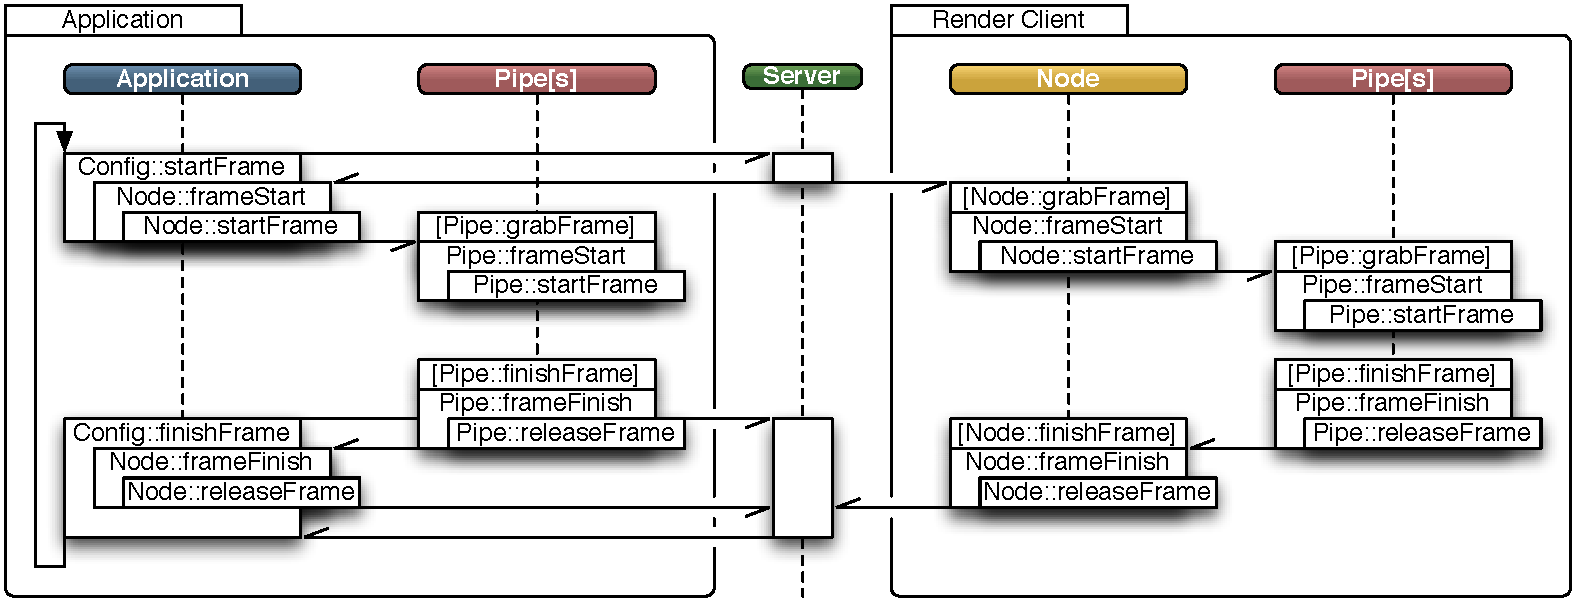
\includegraphics[width=.9\textwidth]{images/mainloop.pdf}
  {\caption{\small\label{fFrameSync}Synchronization of frame tasks}}
\end{figure}

\fig{fFrameSync} outlines the synchronization for the application, node
and pipe classes. The window and channel synchronization is similar and
omitted for simplicity. The \textsf{eqPly} example does not override
\textsf{Node::frameStart} or \textsf{frameFinish}, but it is absolutely
vital for the execution that \textsf{Node::startFrame} or
\textsf{Node::finishFrame} are called, respectively. The default
implementation of the node task methods does take care of that.

\subsection{Pipe}

All task methods for a pipe and its children are executed in a separate
thread. This approach optimizes usage of the GPU resource, since all
tasks are executed serially and do not compete for the usage, i.e.,
context switches are minimized. Later versions of Equalizer might
introduce threaded windows to allow the parallel and independent
execution of rendering tasks on a single pipe.

\subsubsection{Initialization and Exit}

Pipe threads are not explicitely synchronized with each other, that is,
pipes might be rendering different frames at one given time. Therefore
frame-specific data has to be allocated for each pipe thread, which in
the \textsf{eqPly} example is the frame data. The frame data is a member
variable of the \textsf{eqPly::Pipe}, and is mapped to the identifier
provided by the initialization data. The initialization in
\textsf{eq::Pipe} does GPU-specific initialization, e.g., the display
connection is opened when glX/X11 is used:

{\footnotesize\begin{lstlisting}
bool Pipe::configInit( const uint32_t initID )
{
    const Node*     node        = static_cast<Node*>( getNode( ));
    const InitData& initData    = node->getInitData();
    const uint32_t  frameDataID = initData.getFrameDataID();
    eq::Config*     config      = getConfig();

    const bool mapped = config->mapObject( &_frameData, frameDataID );
    EQASSERT( mapped );

    return eq::Pipe::configInit( initID );
}
\end{lstlisting}}

The config exit is again symmetric to the config initialization. The
frame data is unmapped and GPU-specific data is de-initialized by
\textsf{eq::Config::exit}:

{\footnotesize\begin{lstlisting}
bool Pipe::configExit()
{
    eq::Config* config = getConfig();
    config->unmapObject( &_frameData );

    return eq::Pipe::configExit();
}
\end{lstlisting}}

\subsubsection{Window System}

Equalizer supports multiple window system interfaces, at the moment
glX/X11, WGL and AGL/Carbon. Some operating systems, and therefore some
Equalizer versions, support multiple window systems\footnote{see
  \link{http://www.equalizergraphics.com/compatibility.html}}.

Each pipe might use a different window system for rendering, which is
determined before \textsf{Pipe::configInit} by
\textsf{Pipe::selectWindowSystem}. The default implementation of
\textsf{selectWindowSystem} loops over all window systems and returns
the first supported window system, determined using
\textsf{supportsWindowSystem}.

The \textsf{eqPly} examples allows selecting the window system using a
command line option. Therefore the implementation of
\textsf{selectWindowSystem} is overwritten, and return the specified
window system, if it is valid:

{\footnotesize\begin{lstlisting}
eq::WindowSystem Pipe::selectWindowSystem() const
{
    const Node*            node     = static_cast<Node*>( getNode( ));
    const InitData&        initData = node->getInitData();
    const eq::WindowSystem ws       = initData.getWindowSystem();

    if( ws == eq::WINDOW_SYSTEM_NONE )
        return eq::Pipe::selectWindowSystem();
    if( !supportsWindowSystem( ws ))
    {
        EQWARN << "Window system " << ws 
               << " not supported, using default window system" << endl;
        return eq::Pipe::selectWindowSystem();
    }

    return ws;
}
\end{lstlisting}}%>>

\subsubsection{Frame Control}

All task methods for a given frame of the pipe, window and channel
entities belonging to the thread are executed in one block, starting
with \textsf{Pipe::frameStart} and finished by
\textsf{Pipe::finishFrame}. The frame start callback is therefore the
natural place to update all frame-specific data to the version belonging
to the frame. 

In \textsf{eqPly}, the version of the only frame-specific object
\textsf{FrameData} is passed as the per-frame id from
\textsf{Config::startFrame} to the frame task methods. The pipe uses
this version to update its instance of the frame data to the current
version, and then unlocks its child entities by calling
\textsf{startFrame}:

{\footnotesize\begin{lstlisting}
void Pipe::frameStart( const uint32_t frameID, const uint32_t frameNumber )
{
    _frameData.sync( frameID );
    startFrame( frameNumber );
}
\end{lstlisting}}


\subsection{Window}

The Equalizer window holds an OpenGL drawable and rendering
context. Subclassed windows should maintain all data specific to the
OpenGL context. The Equalizer window creation routines share the OpenGL
context with the first window of the pipe, this allowing the reuse of
OpenGL objects, e.g., display lists and textures.

\subsubsection{Initialization and Exit}

\begin{wrapfigure}{r}{.4\textwidth}
  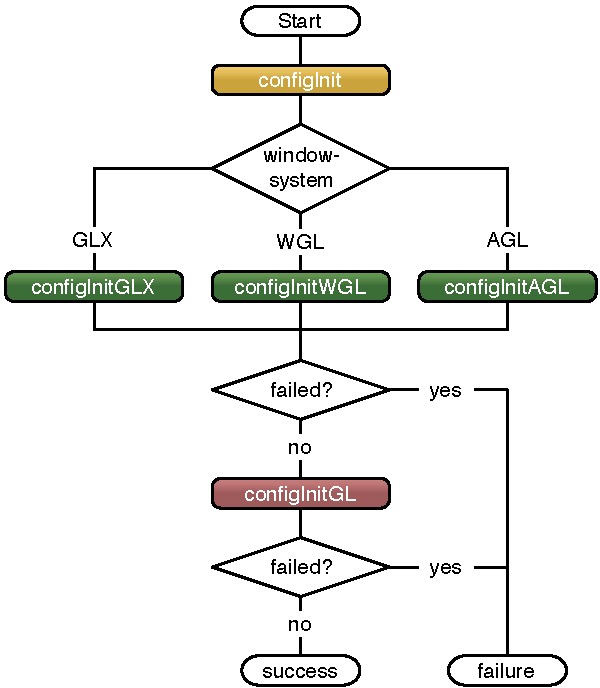
\includegraphics[width=.4\textwidth]{images/windowInit.pdf}
  {\caption{\small\label{fWindowInit}Window Initialization}}
\end{wrapfigure}

The initialization sequence uses multiple, overrideable task
methods. The main task method \textsf{configInit} executes a `child'
task method to create the drawable and context. The child task method
depends on the pipe's window system. The default implementations
\textsf{configInitGLX}, \textsf{configInitWGL} or \textsf{configInitAGL}
create an on-screen window using OS-specific methods. If the OpenGL
drawable and context was created successfully, \textsf{configInit} calls
\textsf{configInitGL}, which performs the generic OpenGL state
initialization. The default implementation sets up some typical OpenGL
state, e.g., it enables the depth test.

\fig{fWindowInit} shows a flow chart of the window initialization. The
colored functions are task methods and can be replaced by
application-specific implementations.

The window-system specific initialization takes into account various
attributes set in the configuration file. Attributes include the size of
various frame buffer attachments (color, alpha, depth, stencil) as well
as other framebuffer properties, such as quad-buffered stereo,
doublebuffering, fullscreen mode and window decorations. Some of the
attributes, such as stereo, doublebuffer and stencil can be set to
\textsf{eq::AUTO}, in which case the default implementation tries to use
them and gradually backs off upon failure.

The \textsf{eqPly} window initialization function first calls
\textsf{eq::Window::configInit} to use the generic window setup. If that
was successful, it initializes a state object and an overlay logo:

{\footnotesize\begin{lstlisting}
bool Window::configInit( const uint32_t initID )
{
    if( !eq::Window::configInit( initID ))
        return false;

    eq::Pipe*  pipe        = getPipe();
    Window*    firstWindow = static_cast< Window* >( pipe->getWindow( 0 ));

    EQASSERT( !_state );

    if( firstWindow == this )
    {
        _state = new VertexBufferState( getGLFunctions( ));
        _loadLogo();

        const Node*     node     = static_cast< const Node* >( getNode( ));
        const InitData& initData = node->getInitData();

        if( initData.useVBOs() )
        {
            const eq::GLFunctions* glFunctions = getGLFunctions();
            // Check if all VBO funcs available, else leave DISPLAY_LIST_MODE on
            if( glFunctions->hasGenBuffers() && glFunctions->hasBindBuffer() &&
                glFunctions->hasBufferData() && glFunctions->hasDeleteBuffers())
            {
                _state->setRenderMode( mesh::BUFFER_OBJECT_MODE );
                EQINFO << "VBO rendering enabled" << endl;
            }
            else
                EQWARN << "VBO function pointers missing, using display lists" 
                       << endl;
        }
    }
    else
    {
        _state       = firstWindow->_state;
        _logoTexture = firstWindow->_logoTexture;
        _logoSize    = firstWindow->_logoSize;
    }

    if( !_state ) // happens if first window failed to initialize
        return false;
    
    return true;
}
\end{lstlisting}}%>>

The state object is used to handle the creation of OpenGL objects in a
multipipe, multi-threaded execution environment. It uses an object
manager, which is described in detail below. It is used in conjunction
with a reference pointer here, since it is potentially `owned' by
multiple windows at the same time.

The logo texture is loaded from the file system and bound to a texture
ID used later by the channel for rendering. The details of this code are
omitted here, since they are pretty straight-forward and not
Equalizer-specific.

The window exit deallocates all OpenGL objects if the state object is
about to be disposed. The object manager does not delete the object in
its destructor, since it does not know if an OpenGL context is still
current. In any case, \textsf{eq::Window::configExit} is called to
destroy the drawable and context:

{\footnotesize\begin{lstlisting}
bool Window::configExit()
{
    if( _state.isValid() && _state->getRefCount() == 1 )
        _state->deleteAll();

    _state = 0;
    return eq::Window::configExit();
}
\end{lstlisting}}

\subsubsection{Object Manager}

The object manager is --strictly speaking-- not part of the window. It
is discussed here since the \textsf{eqPly} window uses an object manager.

The state object in \textsf{eqPly} gathers all rendering state, which
includes an object manager for object state handling. This state object
can easily be replaced to use the rendering code in a stand-alone
application, e.g., for an GLUT-based renderer.

The object manager (OM) is a utility class and can be used to manage
OpenGL objects across shared contexts. Typically one OM is used for each
set of shared contexts, which normally spawns all contexts of a single
GPU\footnote{\link{http://www.equalizergraphics.com/documents/design/objectManager.html}}.

The OM is a template class. The template type is the key type, by which
objects can be identified. The same key is used by all contexts to get
the OpenGL name of an object. In \textsf{eqPly}, a key of type
\textsf{const void *} is used. The rendering code uses the address of
the data item to be rendered to obtain the associated OpenGL object.

The usage of objects is reference counted. If an application releases
the objects properly, they are automatically de-allocated. It is also
possible to manually manage de-allocation of objects, which is often the
more convenient use case.

Currently handling for display lists, textures and buffers is
implemented. For each object, the following functions are available:

\begin{description}
\item[supportsObjects()]: returns true if the usage for this particular
  type of objects is supported. For basic objects, which are supported
  on all OpenGL implementations, this function is not implemented.
\item[getObject( key )]: returns the object associated with the given
  key, or FAILED. Increases the reference count of existing objects.
\item[newObject( key )]: allocates a new object for the given
  key. Returns FAILED if the object already exists or if the allocation
  failed. Sets the reference count of a newly created object to one.
\item[obtainObject( key )]: convenience function which gets or obtains
  the object associated with the given key. Returns FAILED only if the
  object allocation failed.
\item[releaseObject( key \textbar\ name )]: decreases the reference count and
  deletes the object if the reference count reaches zero.
\item[deleteObject( key \textbar\ name )]: manually deletes the object. To be
  used if reference counting is not used.
\end{description}


\subsection{Channel}

The channel is the heart of the application in that it contains the
actual rendering code. The channel is used to perform various rendering
operations.

\subsubsection{Initialization and Exit}

During channel initialization, the near and far planes are set to
reasonable values to contain the whole model. During rendering, the near
and far planes are adjusted to the current model position:

{\footnotesize\begin{lstlisting}
bool Channel::configInit( const uint32_t initID )
{
    setNearFar( 0.1f, 10.0f );
    return true;
}
\end{lstlisting}}

\subsubsection{Rendering}

The central rendering routine is \textsf{Channel::frameDraw}. This
routine contains the application's OpenGL rendering code, which is being
rendered using the rendering context provided by Equalizer. 

In \textsf{eqPly}, the OpenGL context is first set up using various
\textsf{apply} convenience methods from the base Equalizer channel
class. Each of the \textsf{apply} methods uses the corresponding
\textsf{get} method(s) and then calls the approriate OpenGL
function(s). It is also possible to just query the values from Equalizer
using the \textsf{get} methods, and use them to set up the OpenGL state
appropriatly, for example by passing the parameters to the renderer used
by the application.

For example, the implementation for \textsf{eq::Channel::applyBuffer}
does set up the correct rendering buffer and color mask, which depends
on the current eye pass and possible anaglyphic stereo parameters:

{\footnotesize\begin{lstlisting}
void eq::Channel::applyBuffer()
{
    glReadBuffer( getReadBuffer( ));
    glDrawBuffer( getDrawBuffer( ));
    
    const ColorMask& colorMask = getDrawBufferMask();
    glColorMask( colorMask.red, colorMask.green, colorMask.blue, true );
}
\end{lstlisting}}

The following contextual information has to be used in order to render
the view expected by Equalizer:
\begin{description}
\item[Buffer]: The OpenGL read and draw buffer as well as color mask.
  These parameters are influenced by the current eye pass, eye
  seperation and anaglyphic stereo settings.
\item[Viewport]: The two-dimensional pixel viewport restricting the
  rendering area within the channel. For correct operations, both
  \textsf{glViewport} and \textsf{glScissor} have to be used. The pixel
  viewport is influenced by the destination channel's viewport
  definition and compound viewports set for sort-first/2D decompositions.
\item[Frustum]: Frustum parameters as defined by
  \textsf{glFrustum}. The frustum is influenced by the destination
  channel's view definition, compound viewports, head matrix and the
  current eye pass.
\item[Head Transformation:] A transformation matrix positioning the
  frustum. This is typically an identity matrix and is used for off-axis
  frustra in immersive rendering.
\item[Range]: A one-dimensional range with the interval [0..1]. This
  parameter is optional and should be used by the application to render
  only the appropriate subset of its data.
\end{description}

Consequently, the first part of the \textsf{frameDraw} method in
\textsf{eqPly} look as follows:

{\footnotesize\begin{lstlisting}
void Channel::frameDraw( const uint32_t frameID )
{
    applyBuffer();
    applyViewport();
            
    glMatrixMode( GL_PROJECTION );
    glLoadIdentity();

    applyFrustum();

    glMatrixMode( GL_MODELVIEW );
    glLoadIdentity();
    applyHeadTransform();
\end{lstlisting}}

\begin{wrapfigure}{r}{.4\textwidth}
  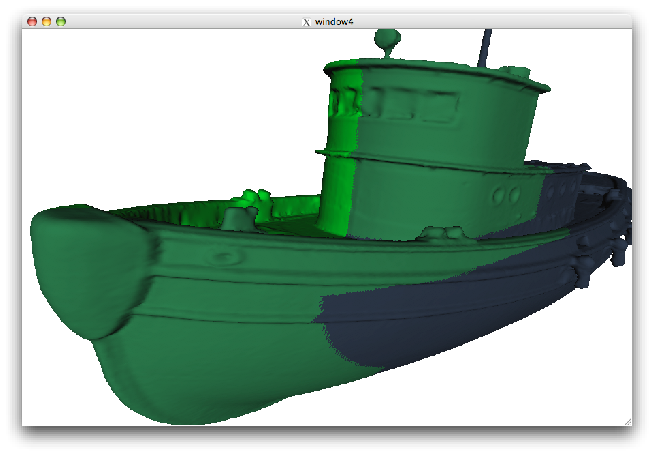
\includegraphics[width=.4\textwidth]{images/DB.pdf}
  {\caption{\small\label{fDB}Final view of an DB compound}}
\end{wrapfigure}

After the basic view setup, a directional light is set up, and the model
is positioned using the camera parameters from the frame data. The
camera parameters are transported using the the frame data to ensure
that all channels render the frame from the same position. 

Furthermore, a color is set in case the model does not contain color
information, or the color information is not to be used. In sort-last
rendering, \textsf{eqPly} renders the individual parts with different
colors to illustrate the algorithm, as shown in \fig{fDB}. The Equalizer
channel provides a method to obtain a random, but unique color for all
channels in the configuration:

{\footnotesize\begin{lstlisting}
    glLightfv( GL_LIGHT0, GL_POSITION, lightpos );

    const Pipe*      pipe      = static_cast<Pipe*>( getPipe( ));
    const FrameData& frameData = pipe->getFrameData();

    glTranslatef( frameData.data.translation.x,
                  frameData.data.translation.y,
                  frameData.data.translation.z );
    glMultMatrixf( frameData.data.rotation.ml );

    Node*            node  = (Node*)getNode();
    const Model*     model = node->getModel();
    const eq::Range& range = getRange();

    if( !range.isFull( )) // Color DB-patches
    {
        const vmml::Vector3ub color = getUniqueColor();
        glColor3ub( color.r, color.g, color.b );
    }
    else if( !frameData.data.color || (model && !model->hasColors( )) )
    {
        glColor3f( 1.0f, 1.0f, 1.0f );
    }
    
\end{lstlisting}}

Finally the model is rendered, if it could be loaded during
initialization. Otherwise a quad is drawn in its place:

{\footnotesize\begin{lstlisting}
    if( model )
    {
        _drawModel( model );
    }
    else
    {
        glColor3f( 1.f, 1.f, 0.f );
        glNormal3f( 0.f, -1.f, 0.f );
        glBegin( GL_TRIANGLE_STRIP );
        glVertex3f(  .25f, 0.f,  .25f );
        glVertex3f(  .25f, 0.f, -.25f );
        glVertex3f( -.25f, 0.f,  .25f );
        glVertex3f( -.25f, 0.f, -.25f );
        glEnd();
    }
}
\end{lstlisting}}

\if 0
{\footnotesize\begin{lstlisting}
void Channel::_drawModel( const Model* model )
{
    Window*                  window    = static_cast<Window*>( getWindow() );
    mesh::VertexBufferState& state     = window->getState();

    const Pipe*              pipe      = static_cast<Pipe*>( getPipe( ));
    const FrameData&         frameData = pipe->getFrameData();

    const eq::Range&         range     = getRange();
    vmml::FrustumCullerf     culler;

    state.setColors( frameData.data.color && 
                     range.isFull() && 
                     model->hasColors() );
    _initFrustum( culler, model->getBoundingSphere( ));

    model->beginRendering( state );
        
\end{lstlisting}}

{\footnotesize\begin{lstlisting}
\end{lstlisting}}

The model data is organized a in 3-dimensional kD-tree\footnote{See also
  \link{http://en.wikipedia.org/wiki/Kd-tree}} for efficient view
frustum culling. During preprocessing, each node of the tree gets a
database range assigned.

{\footnotesize\begin{lstlisting}
\end{lstlisting}}
\fi

\section{Advanced Features}

This section discusses some features of interest which are not covered
by the \textsf{eqPly} section. Where possible, code examples from the
Equalizer distribution are used.


\subsection{Event Handling}

Event handling is one of the areas which requires a lot of
flexibility. On one hand, the implementation differs slightly for each
window system due to conceptual differences in the OS-specific
implementation. On the other hand, each application and widget set has
its own model on how events are to be handled. Therefore, event handling
in Equalizer is customizable in any stage of the processing\footnote{\link{http://www.equalizergraphics.com/documents/design/eventHandling.html}}. 

The default implementation aims to provide a quick and easy
implementation of event handling, while allowing all necessary
customizations. It gathers all events in the application main thread, so
that the developer only has to implement \textsf{Config::processEvent}
to update its data based on the pre-processed, generic events.


\subsubsection{Threading}

Where possible, events are received and processed by a separate per-node
event thread to allow asynchronous event handling. Currently an event
thread is only used by the X11/glX window system. WGL receives and
processes the events from the pipe threads which created the
windows. AGL receives the events from application or node main
thread. Whenever the term \textbf{event thread} is used, it refers to
the thread receiving the event, i.e., a per-node thread for glX, the pipe
thread for WGL and the main thread for AGL.

\subsubsection{Initialization and Exit}

\begin{wrapfigure}{r}{.4\textwidth}
  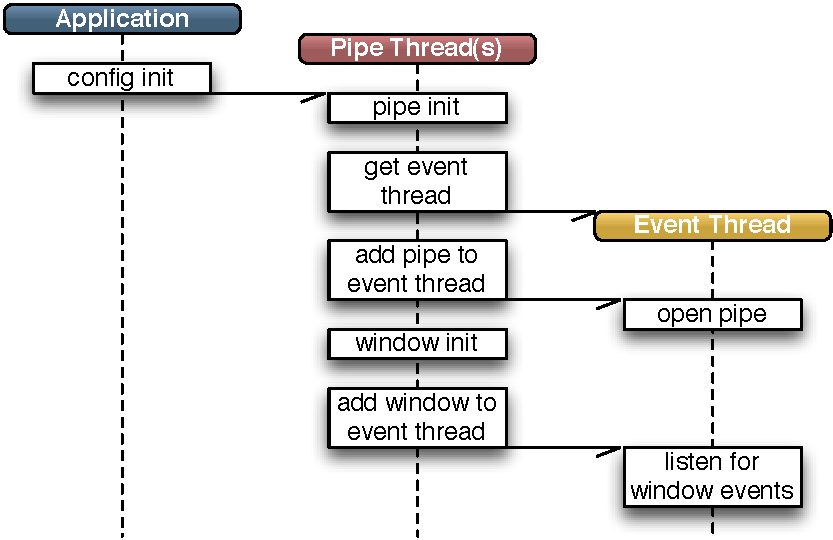
\includegraphics[width=.4\textwidth]{images/eventInit.pdf}
  {\caption{\small\label{fEventInit}Event Handling Initialization}}
\end{wrapfigure}

During window and pipe initialization the event handling is set up. For
both entities, \textsf{initEvent\-Handler} is called to register the pipe
or window with an event handler. This method may be overwritten to use a
custom event handler, or to not install an event handler to disable
event handling in Equalizer. Likewise, \textsf{exitEventHandler} is
called to de-initialize event handling.

An event handler consists of two parts: the generic base class providing
the interface and some generic functions, and the window-system-specific
part providiing the actual implementation. 

Pipe event handling is only used for glX, where one \textsf{Display}
connection is created to subscribe to window events. Event handling is
initialized whenever a new, window-system-specific pipe or window handle
is set. First, \textsf{exitEventHandler} is called to de-initialize
event handling for the old handle (if set), and then
\textsf{initEvent\-Handler} is called for the new handle. AGL and glX use
an event handler singleton, whereas WGL uses one event handler per
window.

\subsubsection{Message Pump}

WGL and AGL require the application to manually receive and dispatch
(`pump') events. On WGL, this has to happen on each thread with windows,
whereas on AGL it has to happen only on the main thread. By default,
Equalizer pumps these events automatically for the application.

The methods \textsf{Client::useMessagePump} and
\textsf{Pipe::useMessagePump} can be overriden to return \textsf{false}
to disable this behaviour for their respective threads. On non-threaded
pipes, \textsf{Pipe::useMessagePump} is not called.


\subsubsection{Event Data Flow}

\begin{wrapfigure}{r}{.4\textwidth}
  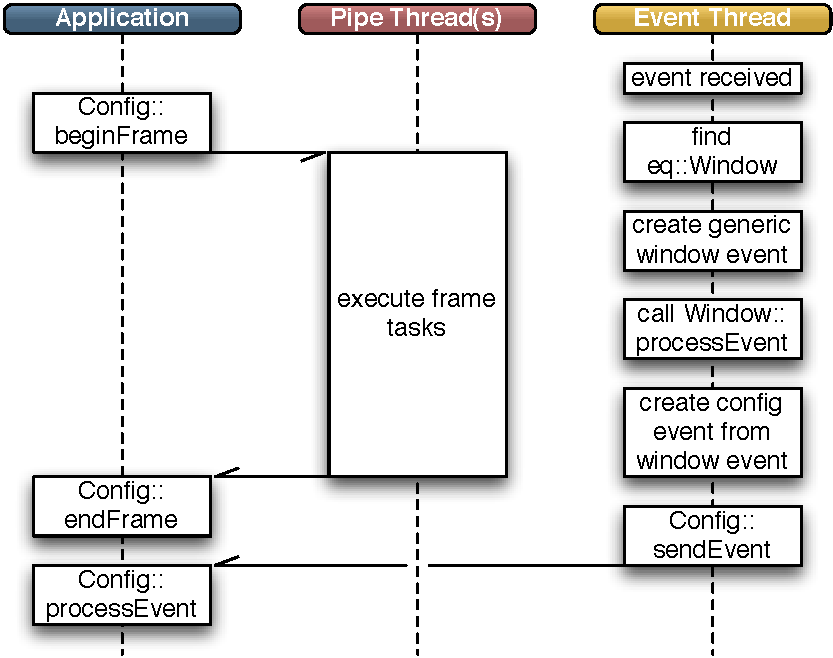
\includegraphics[width=.4\textwidth]{images/eventHandling.pdf}
  {\caption{\small\label{fEventProcessing}Event Processing}}
\end{wrapfigure}

Events are received by an event handler. The event handler finds the
\textsf{eq::Window} associated to the event. It then creates a generic
\textsf{WindowEvent}, which holds important event data in a format
independent of the window system. The original event is attached to the
generic window event.

The event handler then passes the window event to
\textsf{Window::processEvent}, which is responsible for either handling
the event locally, or for translating it into a generic
\textsf{ConfigEvent}. The config events are send to the application
thread using \textsf{Config::sendEvent}. If the event was processed, the
function has to return \textsf{true}. If \textsf{false} is returned, the
event will be passed to a previously installed, window-system-specific
event handling function. The default implementation of
\textsf{Window::processEvent} passes most events on to the application.

Events sent using \textsf{Config::sendEvent} are queued in the
application thread. After a frame has been finished,
\textsf{Config::finishFrame} calls \textsf{Config::processEvents}. The
default implementation of this method provides non-blocking event
processing, that is, it calls \textsf{Config::processEvent} for each
queued event. By overriding this function, event-driven execution can be
implemented.

\subsubsection{Custom Events in eqPixelBench}

The \textsf{eqPixelBench} example is a benchmark program to measure the
pixel transfer rates from and to the framebuffer of all channels within
a configuration. It uses custom config events to send the gathered data
to the application. It is much simpler than the \textsf{eqPly} example
since it does not provide any useful rendering or user interaction.

The rendering routine of \textsf{eqPixelBench} in
\textsf{Channel::frameDraw} loops through a number of pixel formats and
types. For each of them, it measures the time to readback and assemble a
full-channel image. The format, type, size and time is recorded in a
config event, which is sent to the application.

The \textsf{ConfigEvent} derives from the \textsf{eq::ConfigEvent}
structure and has the following definition:

{\footnotesize\begin{lstlisting}
struct ConfigEvent : public eq::ConfigEvent
{
public:
    enum Type
    {
        READBACK = eq::ConfigEvent::USER,
        ASSEMBLE
    };

    ConfigEvent()
        {
            size = sizeof( ConfigEvent );
        }

    // channel name is in user event data
    char           formatType[64];
    vmml::Vector2i area;
    float          msec;
};
\end{lstlisting}}

The \textsf{Config::sendEvent} method transmits a
\textsf{eq::ConfigEvent} or derived class to the application. The
ConfigEvent has to be a C-type structure, and its \textsf{size}
member has to be set to the full size of the event to be transmitted.
Each event has a type, by which the config processing function can
identify it. 

User-defined types start at \textsf{eq::ConfigEvent::USER}, and the
member variable \textsf{ConfigEvent::user} can be used to store
\textsf{EQ\_USER\_EVENT\_SIZE}\footnote{currently 32 bytes} bytes. In
this space, the channel's name is stored. Additional variables are used
to transport the pixel format and type, the size and the time it took
for rendering.

On the application end, \textsf{Config::handleEvent} uses the ostream
operator for the derived config event to output these events in a nicely
formatted way:

{\footnotesize\begin{lstlisting}
std::ostream& operator << ( std::ostream& os, const ConfigEvent* event );
...
bool Config::handleEvent( const eq::ConfigEvent* event )
{
    switch( event->type )
    {
        case ConfigEvent::READBACK:
        case ConfigEvent::ASSEMBLE:
            cout << static_cast< const ConfigEvent* >( event ) << endl;
            return true;

        default:
            return eq::Config::handleEvent( event );
    }
}
\end{lstlisting}}%>>


\subsection{Image Compositing for Scalable Rendering}

Two task methods are responsible for collecting and compositing the
result image during scalable rendering, when multiple channels are
rendering for a single view. The source channels producing an
\textsf{outputFrame} use \textsf{Channel::frameReadback} to read the
pixel data from the frame buffer. The channels receiving one or multiple
\textsf{inputFrame} use \textsf{Channel::frameAssemb\-le} to assemble
the frames into the framebuffer. Equalizer takes care of the network
transport of frame buffer data between nodes, if needed.

\subsubsection{Frame, FrameData and Images}

A \textsf{eq::Frame} references a \textsf{eq::Fra\-me\-Data}. The frame data
is the object connecting output with input frames. It is a holder for
images and is used to signal the availability of the pixel data. An
\textsf{eq::Image} holds a two-dimensional snapshot of the framebuffer
and can contain color and/or depth information.

Readback and assemble operations on frames and images are designed to be
asynchronous. They have a start and finish method for readback and
assemble to allow the initiation and synchronization of the operation.
Currently, only synchronous readback and assembly using
\textsf{glReadPixels} and \textsf{glDrawPixels} is implemented in the
respective start method of the image.

\if 0

\begin{wrapfigure}{r}{.6\textwidth}
  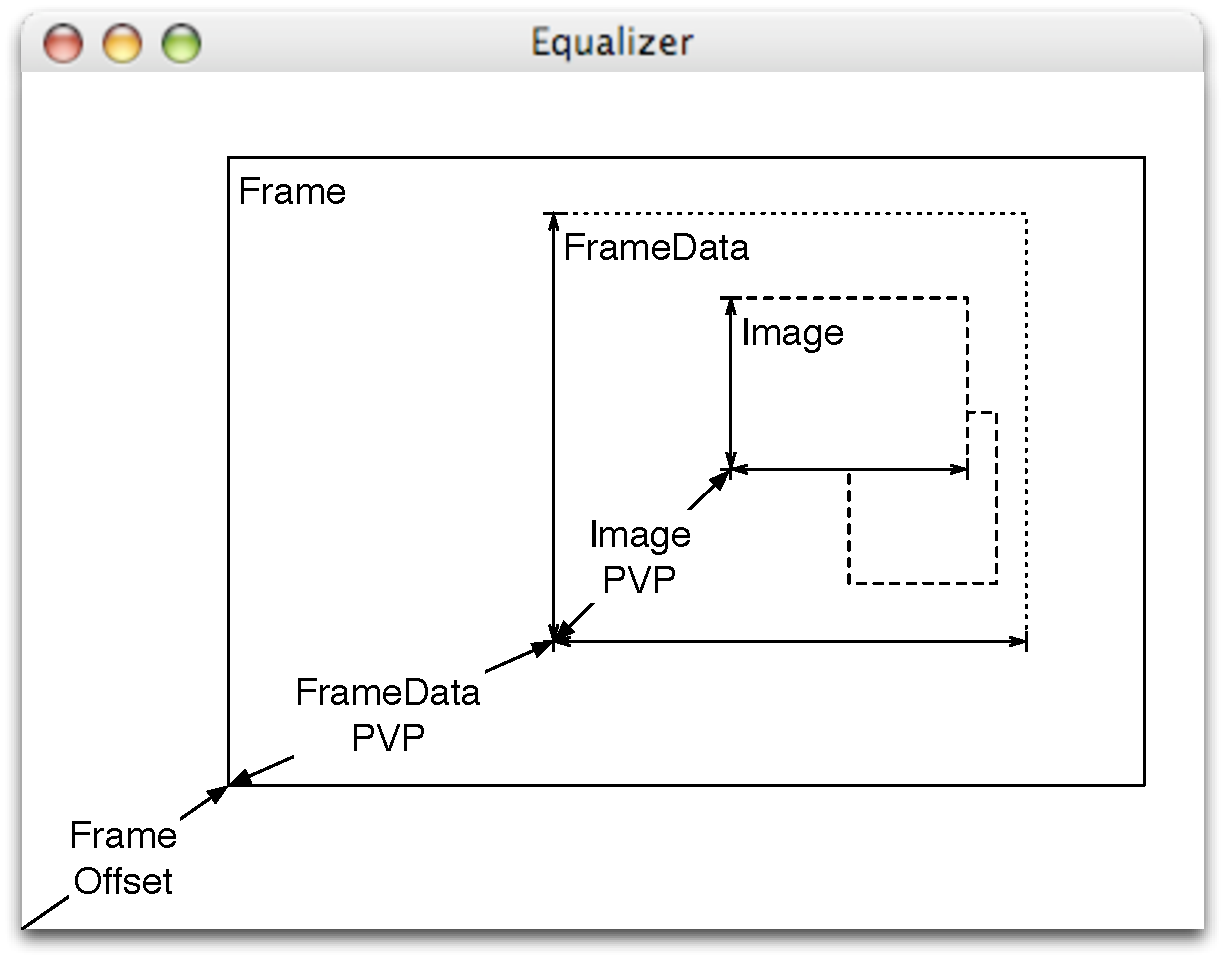
\includegraphics[width=.6\textwidth]{images/assembly.pdf}
  {\caption{\small\label{fAssembly}Hierarchy of assembly classes}}
\end{wrapfigure}

The offset of input and output frames characterizes the position of the
frame data with respect to the framebuffer, that is, the
\textbf{window's} lower-left corner. For output frames this is the
position of the channel in 
\fi

\subsubsection{Custom Assembly in eVolve}


\subsection{Head Tracking}
\if 0
{\footnotesize\begin{lstlisting}
\end{lstlisting}}
\fi

\end{document}
